\documentclass{standalone}
\usepackage[svgnames]{xcolor}
\usepackage{pgfplots}
\begin{document}
  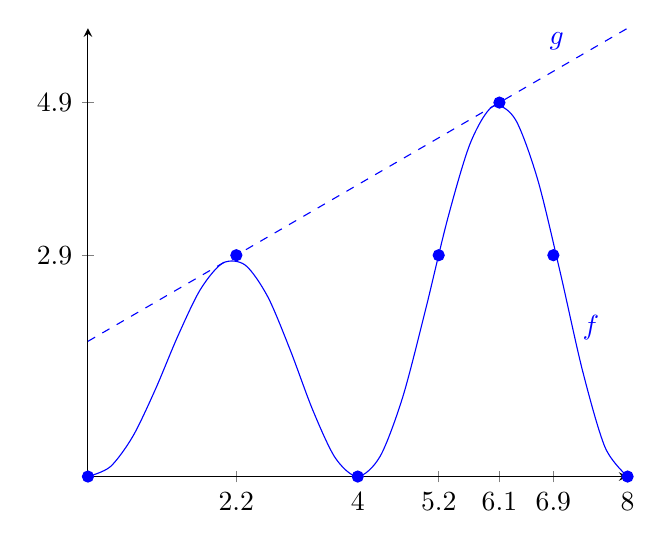
\begin{tikzpicture}
    \begin{axis}[
      axis lines = center,
      xtick = {2.2,4.0,5.2,6.1,6.9,8.0},
      ytick = {2.9,4.9},
    ]
      \addplot[domain=0:8, dashed, color=blue] {0.512820512820513*(x - 2.2) + 2.9} node[above left,pos=0.9] {\(g\)};
      \addplot[domain=0:8, color=blue, smooth] {(0.512820512820513*(x - 2.2) + 2.9)*1/2*(1 - cos(pi/2*deg(x)))} node[right,pos=0.88] {\(f\)};
      \addplot[mark=*, only marks, color=blue] coordinates {(0,0) (2.2,2.9) (4,0) (5.2, 2.9) (6.1, 4.9) (6.9, 2.9) (8,0)};
    \end{axis}
  \end{tikzpicture}

\end{document}
